\documentclass[12pt,a4paper]{article}
\usepackage[T2A]{fontenc}
\usepackage[utf8x]{inputenc}
\usepackage[english,russian]{babel}
\usepackage{amsmath,amsfonts,amssymb,amsthm,mathtools}
\usepackage{wrapfig}

\author{Коллективный разум}
\title{\textit{Бе}се\textit{ды} с \textit{Ба}тю\textit{шкой}}
\date{\today}

\begin{document}

\maketitle
\newpage

\section*{Гомеоморфизм}

Пусть $M,N \subset \mathbb{R}^{n}.$ $f:M\longrightarrow N$ -- отображение\footnote{Отображение $f:M\rightarrow N$ -- закон, который каждому элементу $x \in M$ ставит в  соответствие единственный элемент $y \in N.$}.\\


Отображение $f$ \textit{непрерывно в точке $a$}, тогда и только тогда, когда 
		\[\lim_{x \to a}{f(x)} = f(a)\]

\textbf{Непрерывность по Коши:}
	\[ 
		\forall \varepsilon > 0 ~
		\exists \delta_{\varepsilon} > 0: ~
		(\forall x\in U_{\delta_{\varepsilon}}(a)\cap M
		\Rightarrow f(x)\in U_{\varepsilon}(f(a))) 
	\]
\begin{center}
	или в многомерном случае
\end{center}
	\[
		\forall \varepsilon > 0	~
		\exists \delta_{\varepsilon} > 0:
		(\forall x\in B_{\delta_{\varepsilon}}(a)
		\Rightarrow \rho(f(x),f(a))<\varepsilon),
		\footnote{
			Здесь ~
			$B_{\delta_{\varepsilon}} = 
			\{y\in \mathbb{R}^n | ~ \rho(y,a) <
			\delta_{\varepsilon}\}$,
			а ~
			$\rho(x,y) = \sqrt{\sum_{i=1}^n(x_i - y_i)^2}$
				}
	\]	
	
	
	\textbf{По Гейне:}
		\[ \forall  x_n \to a \Rightarrow f(x_n) \to f(a) \]\\
	
	\textbf{\large{Определение:}} отображение $f:M \to N$ называется \underline{\textit{гомеоморфизмом}}, если
	\begin{itemize}
		\item $f$ -- биекция,
		\item $f$ -- непрерывна,
		\item $f^{-1}$ -- непрерывна
	\end{itemize}
	Говорят, что $M$ гомеоморфно $N$ и обозначается
	\begin{center}
	$M \cong N$
	\end{center}
	
	
	
	\textbf{\large{Упражнение 1:}} доказать или опровергнуть, что ллюбая нерпрерывная биекция является гомеоморфизмом.
	
	\textbf{\large{Упражнение 2:}} доказать, что $(0,1) \cong  \mathbb{R}$
	
	\textbf{\large{Упражнение 3:}} доказать, что $D\cong \mathbb{R}^2$,
	
	\[ \textit{где}~ D =\{(x,y)\in \mathbb{R}^2 | x^2 + y^2 < 1\} \]
	
	\newpage
\section*{Многообразие}

Пусть \(M \subset \mathbb{R}^n\) такое, что \(\exists k\in \mathbb{N}\), $\forall \varepsilon >0$:
\begin{center}
 \textit{либо} \(U_{\varepsilon} (x)\cap M \cong \mathbb{R}^k\),
\end{center}
\begin{center}
 \textit{либо} \(U_{\varepsilon} (x)\cap M \cong \mathbb{R}_{+}^k\),
\end{center}
\textit{где} \(\mathbb{R}_{+}^k = \{(x_1,x_2,...,x_k)|~ x_1,..., x_{k-1} \in \mathbb{R}, x_k\ge 0\}\)
\newline в этом случае M является \underline{\textbf{многообразием}} размерности k.
\newline Если \(\nexists\) окрестности \(U_{\varepsilon} (x): U_{\varepsilon} (x)\cap M \cong \mathbb{R}^k\), то \(x\) - \textbf{граничная точка}, иначе \(х\)- \textbf{внутренняя точка}.
\newline Если множество граничных точек пустое (\(\emptyset\)), то \(M\)- многообразие \textbf{без края}, в противном случае \textbf{с краем}.
\newline \textbf{Примеры:}
\newline 1. Диск: $D^1 = \{(x,y) \in \mathbb{R}^2 |~ x^2 + y^2 < 1 \} $
\newline 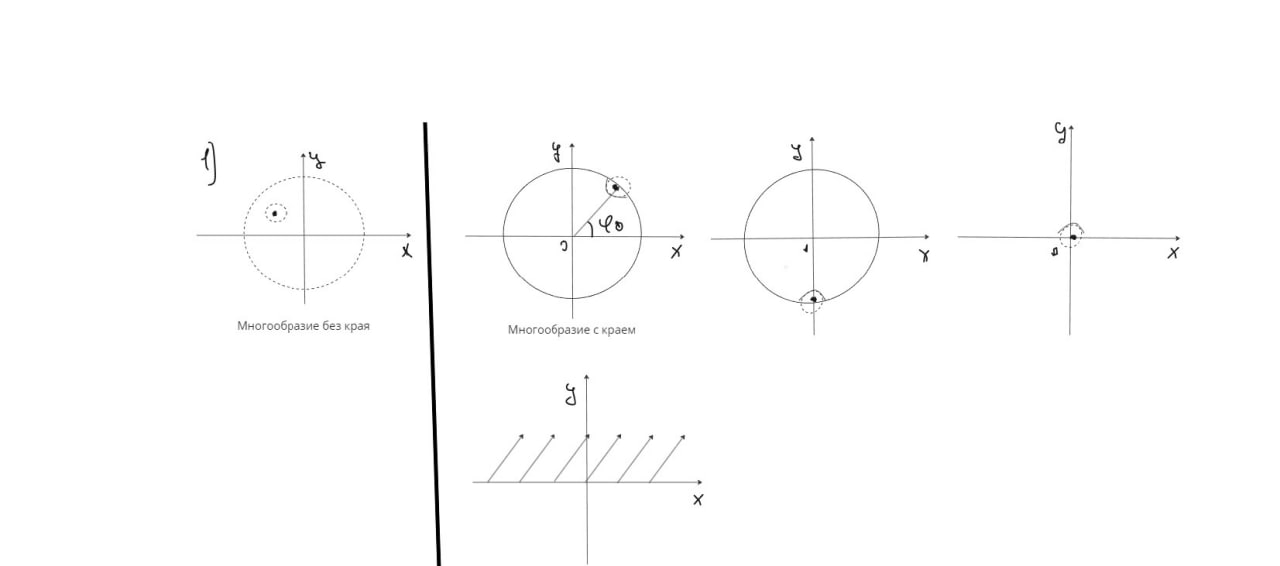
\includegraphics[scale=0.7]{images/Section 2. Manifold/image1}
\newline 2. Окружность: \(S^1 = \{(x,y)\in \mathbb{R}^2|~ x^2 + y^2 =1\}\) 
\newline 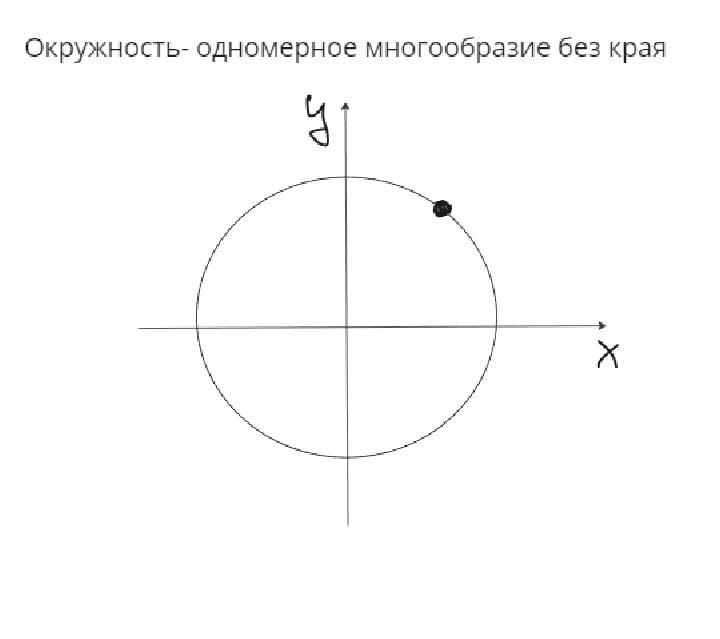
\includegraphics[scale=0.85]{images/Section 2. Manifold/image2}
\newpage 3. Сфера: \(S^2 = \{(x,y,z)\in\mathbb{R}^3|~ x^2+y^2+z^2=1\}\)
\newline 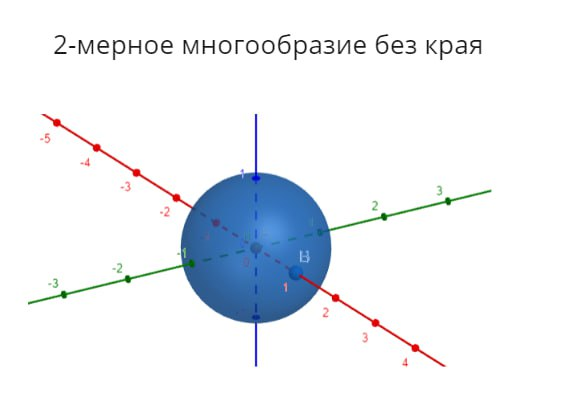
\includegraphics[scale=0.5]{images/Section 2. Manifold/image3}
\newline 4. Тор. Рассматриваем как поворот единичной окружности вокруг оси Oz.
\(T=\{(x,y,z)\in \mathbb{R}^3\)|
\begin{equation*}
\begin{cases}
(y - 2)^2 + z^2=1
\\
x =0
\end{cases}
\end{equation*}
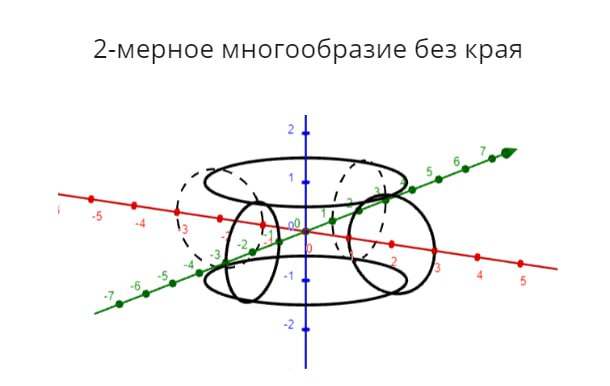
\includegraphics[scale=0.5]{images/Section 2. Manifold/image4}\\

5. Цилиндр.
\newline \(C = \{(x,y,z)\in \mathbb{R}^3\)|
\begin{equation*}
\begin{cases}
x^2+y^2=1
\\
0\leq z\leq1 
\end{cases}
\end{equation*}
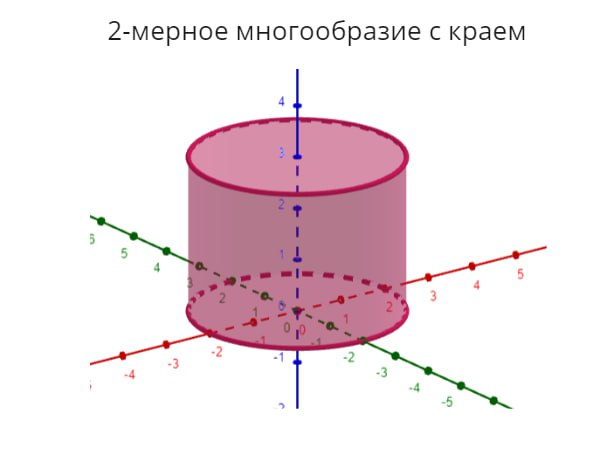
\includegraphics[scale=0.5]{images/Section 2. Manifold/image5}
\newpage

\section*{Динамическая система}

\textbf{\large{Определение:}} Пусть M -- многообразие. \textbf{Динамической системой(ДС)} 
на многообразии M называется непрерывное отображение $f:M\times X \rightarrow M~$ $(X = \mathbb{R}~ \textit{или}~ X = \mathbb{Z})$ со следующими свойствами:

\begin{enumerate}
\item $f(x,0) = x,\qquad \forall x \in M$
\item $f(f(x,t),s) = f(x, t+s),\qquad \forall x \in M \forall t,s \in X$ 
\end{enumerate} 

Если $X = \mathbb{R}$, то ДС называется \textbf{потоком} (непрерывная ДС).
Если $X = \mathbb{Z}$, то ДС называется \textbf{каскадом} (дискретная ДС).\\

Динамическая система $f:M\times X: \rightarrow M$ определяет семейство гомеоморфизмов $\{ f^t~|~ t \in \mathbb{R}(\mathbb{Z}) \}$ на M, где $f^t(x) \equiv f(x,t)$. \\

Если $t \in \mathbb{Z}$, то
\begin{itemize}
\item при $t > 0 \qquad f^t = \underbrace{f \circ \ldots \circ f}_t$;
\item при $t < 0 \qquad f^t = \underbrace{f^{-1} \circ \ldots \circ f^{-1}}_t$;
\item $f^0 = Id:M \rightarrow M, ~~ Id(x) = x$
\end{itemize}

\textbf{\large{Определение:}} \textbf{Траекторией} точки $x_0 \in M$ называется множество $O_{x_0} = \{f^t(x_0)~|~ t \in \mathbb{R(\mathbb{Z}} \}$. Если $t \in \mathbb{Z}$, то траекторию называют \textbf{орбитой}.\\

\textbf{Пример 1.} 
$x_t = v_0\cdot t + x_0,$

$~ t\in \mathbb{R};$\\

$f^t:\mathbb{R} \rightarrow \mathbb{R};$\\

$f^t(x_0) = v\cdot t.$
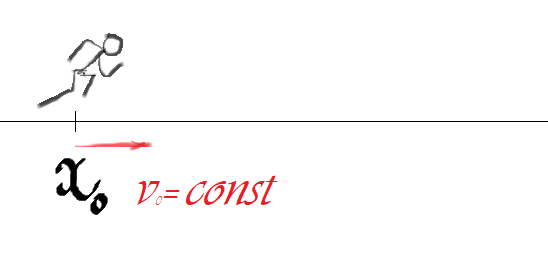
\includegraphics[scale = 0.45]{images/Section 3. Dinamic System/runner}
\newpage \textbf{Пример 2. Математический маятник без трения} 
$ (\alpha ,V_x)$

$\alpha \in [-\pi , \pi]$

$0\sim 2\pi$
$V_x \in \mathbb{R}$


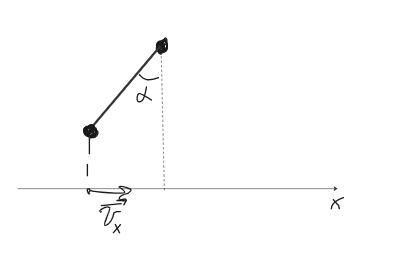
\includegraphics[scale=0.5]{images/Section 3. Dinamic System/image12}
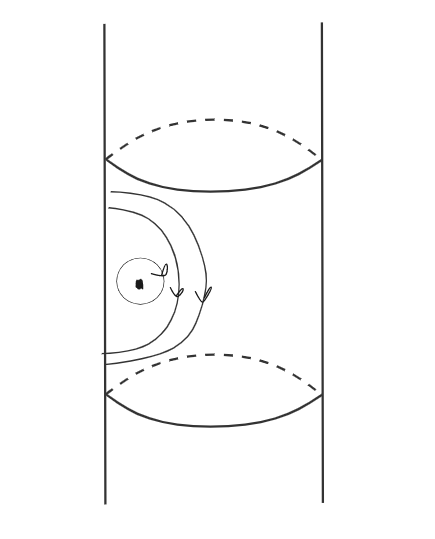
\includegraphics[scale=0.3]{images/Section 3. Dinamic System/image6}
\newline
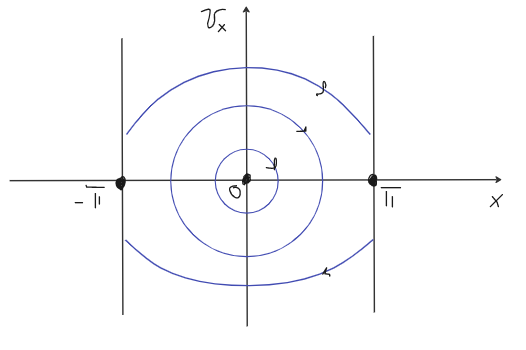
\includegraphics[scale=0.4]{images/Section 3. Dinamic System/image7}
 \newpage \textbf{Пример 3. Математический маятник с трением.}


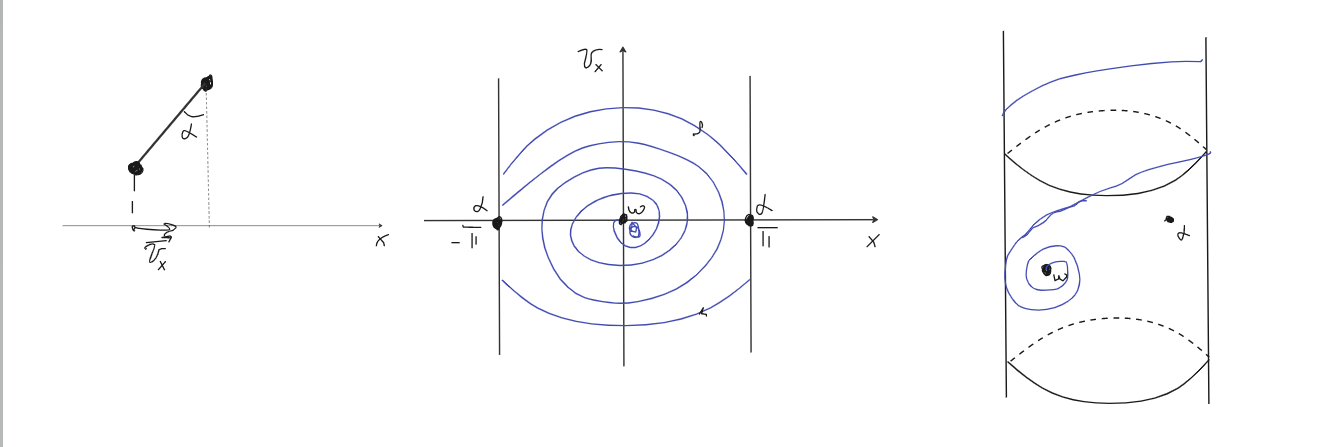
\includegraphics[scale=0.3]{images/Section 3. Dinamic System/allimage}
\newline
\textbf{Определение:} Точка \(x\in M\) называется блуждающей, если \(\exists U(x)\) и \(\exists T : \forall t >T \rightarrow f^t(U(x))\cap U(x) = \varnothing\) 
\newline В противном случае, точка называется неблуждащей.
\newline \textbf{Определение:} Объединение неблуждающих точек - неблуждающее множество.
\newline \textbf{Определение: } Неподвижная точка - точка,траектория которой совпадает с ней (\(O_x = \{x\}\)).
\newline \textbf{Обозначения: } \(\omega\) - сток (притягивающая неподвижная точка)
\newline \(\alpha\) - источник (отталкивающая неподвижная точка)
\newline \textbf{Определение: } \(x \in M\) -периодическая для потока \(f^t\) (каскад f), если \(\exists T > 0: f^T(x)=x \forall \\ 1<t_1 <T  \\ f^{t_1}(x)\neq x\)
\newline \textbf{Примеры: Каскады}
\newline \textbf{Обозначение: } \(NB(f)=\{...\}\)- множество неблуждающих точек.
\\
\newline 1. \(f(x)= \bar{x}=0,5 x \\ t\in \mathbb{Z}, f^t= \underbrace{f \circ \ldots \circ f}_t\) 
\newline 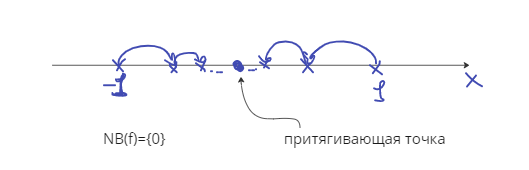
\includegraphics[scale=0.5]{kaskad1.png}
\\
\newpage 2. \(f(x)=2x\) 
\newline 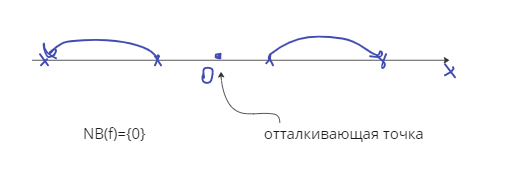
\includegraphics[scale=0.5]{kaskad2.png}
\\
\newline 3. \(f(x)=x+\alpha \\ \alpha \in \mathbb{R}\) 
\newline 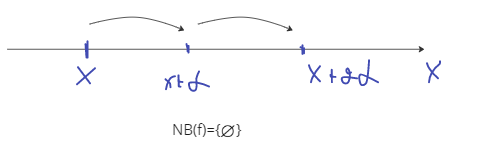
\includegraphics[scale=0.5]{kaskad3.png}
\newline Построим стереометрическию проекцию функций 1, 2, 3
\newline 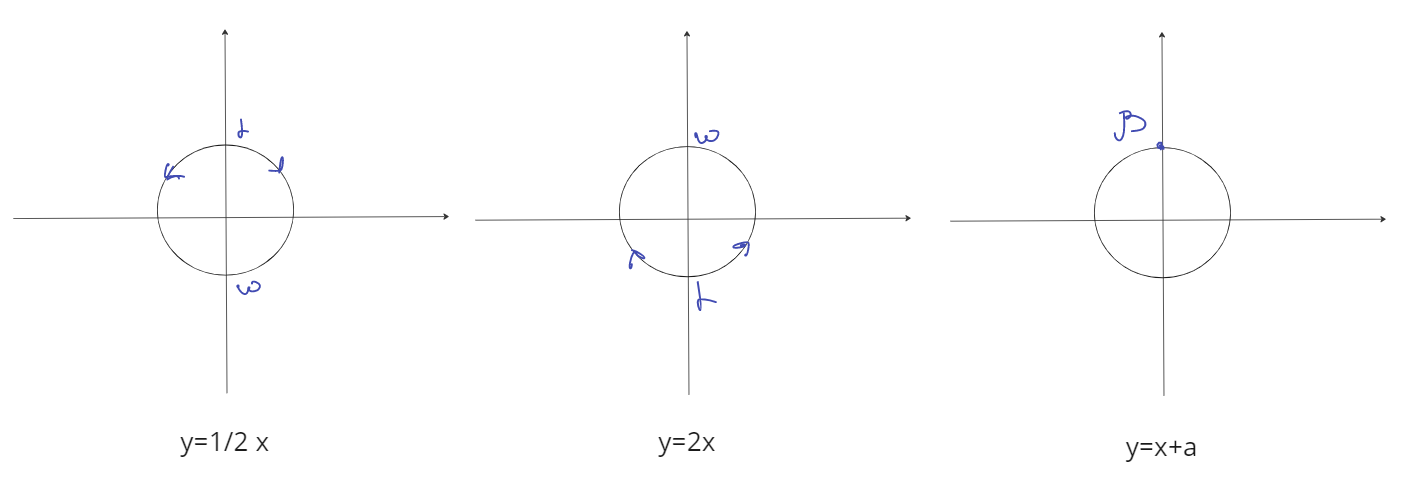
\includegraphics[scale=0.3]{stereo.png}
\newpage
 \section*{\(\varepsilon\) -траектория и и цепно-рекурентное множество.}
 \(O_x=\{f^t(x)|t\in \mathbb{R}(\mathbb{Z}\}\)\\ \(t \in \mathbb{Z}=\{...,f^{-2}(x), f^{-1},x,f^1(x),...\}\) \\ \(x_0,f(x_0)\to x_1\) (причём \(f(x_0)\) можем точно посчитать) \(|x_1 - f(x_0)|<\epsilon\) 
\\
\(...,x_{-1},x_0,x_1,...,x_n - \epsilon\) - траектория
\\
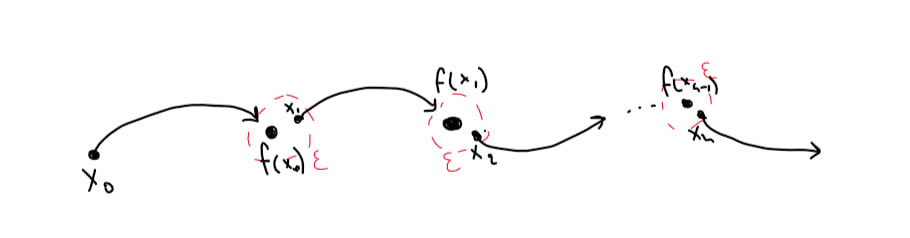
\includegraphics[scale=0.5]{picture.jpg}
\newline \textbf{Определение: } Бесконечный в обе стороны набор точек \(...,x_{-1},x_0,x_1,...\), удовлетворяющий условию \(|x_{k+1} - f(x_k)|<\epsilon\\ \forall k\in \mathbb{Z}\) называется \(\varepsilon\)-траекторией для каскада \(f:M\to M\) 
\newline \(x_0,...,x_n \in M - \varepsilon\)-цепь для каскада f, если \(|x_k - f(x_{k-1})|<\epsilon\) \(\forall k \in 1,2,...,n\)
\newline \textbf{Определение:} Точка \(x \in M\) называется цепно-рекурентной для каскада f, если \(\forall \varepsilon >0 \ \exists\) периодическая \(\varepsilon\)-траектория, проходящая через x.\\
\(\varepsilon\)-траектория - периодическая с преиодом \(T>0\), если \(\forall k\in \mathbb{Z}: \\ x_{k+T} = f^T(x_k)\)\\
Точка \(x \in M\) - цепно-рекурентная для каскада, если \(\forall \varepsilon >0 \exists \varepsilon\)-цепь, соединяющая x саму с собой, т.е. \(x =x_0,...x_n=x\)
\newline \textbf{Определение: } Множество всех цепно-рекурентных для каскада называется его цепно-рекурентным множеством и обозначается: \(R_f\).
\newline \textbf{Пример 1.}
\\
\(f: S^1 \to S^1\) 
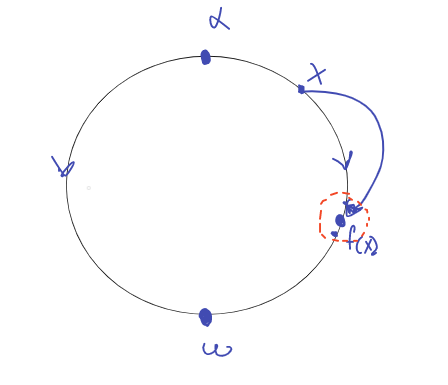
\includegraphics[scale=0.3]{stos.png}
\\
\(R_f =\{\alpha , \omega\}\)\\Пусть \(\varepsilon = {|f(x)-x|\over {2}}\), тогда \(\forall x_1 \in U_{\varepsilon} (f(x)) \ d(x,x_1)> \varepsilon\) 
\\ \(d(x,f(x))> 2\varepsilon \Rightarrow d(x,x_2) >\varepsilon \Rightarrow ... \Rightarrow \forall i \ d(x, x_i)> \varepsilon\) 


\end{document}
